\documentclass[UTF8]{ctexart}
\usepackage{mathtools,wallpaper}
\usepackage{t1enc}
\usepackage{pagecolor}
\usepackage{enumitem}
\usepackage{hyperref}
\usepackage{graphicx}
\usepackage{listings}
\usepackage{amssymb}
\usepackage[dvipsnames]{xcolor}
\usepackage{float}
\usepackage{numerica}



\begin{document}

\section{Chp1}
\subsection{计算机图形学基本定义}
\begin{itemize}
    \item 图形系统由一台配备有快速处理器和大容量内存的主机组成。
    \begin{enumerate}
        \item 显示设备：color monitor
        \item 输入设备：键盘，鼠标，触控屏
        \item 输出设备：LCD panels液晶面板，color printer，laser printer，plotter
        \item 接口设备：
    \end{enumerate}
    \item 图像类型（根据图形的组成）
    \begin{enumerate}
        \item raster graphics
        \begin{itemize}
            \item 光栅图像(也叫bitmap image)是由一系列像素组成的图像，JPEG，PNG，GIF
        \end{itemize}
        \item vector graphics
        \begin{itemize}
            \item mathematical formulas is used for plotting different types of shapes.
        \end{itemize}
    \end{enumerate}
    \item 图像类型（根据图形的控制）
        \begin{enumerate}
        \item Interactive graphics
        \begin{itemize}
            \item 在可交互图像中，用户可以在图像上有一些控制，并且可以对生成的图像做一些改变。
        \end{itemize}
        \item Passive graphics
        \begin{itemize}
            \item 在被动式图像中，用户不可以对展示在显示屏上的图像进行一些控制。
        \end{itemize}
    \end{enumerate}
    \item Application areas of Computer Graphics
        \begin{enumerate}
            \item Computer-aided Design
            \begin{itemize}
                \item Automobiles - wireframe outline shape of an automobiles internal components.
                \item A multi-window environment with different orientation.
                \item Aircraft - wireframe outline for different features.
                \item Real-time Animation for testing performance.
                \item buildings.
                \item textiles.
            \end{itemize}
            \item Presentation Graphics
            \begin{itemize}
                \item Bar charts
                \item Pie charts
                \item Line graphs
                \item Surface graphs
            \end{itemize}
            \item Computer Art
            \begin{itemize}
                \item Cartoon drawing
                \item fine art(e-painting, photography)
                \item commercial art applications(advertising, logo)
            \end{itemize}
            \item Entertainments
            \begin{itemize}
                \item Movies
                \item Short films
                \item TV serials.
            \end{itemize}
            \item Education and Training
            \begin{itemize}
                \item Flight simulator
                \item Simulators for practice sessions.
                \item simulators of military tanks.
            \end{itemize}
            \item Image Processing
            \begin{itemize}
                \item CT scans.
                \item PS,PR application to improve the quality of a picture.
            \end{itemize}
            \item Graphical User Interface GUI
            \begin{itemize}
                \item Clickable buttons.
                \item Dialog box is to display additional information for users.
                \item Icon is a small symbol.
                \item Menu is a list of commands or choices.
            \end{itemize}
            \item Visualization
            \begin{itemize}
                \item Producing graphical representations for scientific, engineering datasets.
                \item Business visualization.
            \end{itemize}
        \end{enumerate}
    \item 计算机图形系统关键组件
    \begin{enumerate}
        \item 输入设备
        \begin{itemize}
            \item Manual data entry devices: Manual input devices are those peripheral devices through which the user can enter the data manually at the time of processing. 键盘，鼠标，joystick，torch screen
            \item Direct data entry devices: Direct data devices are those peripheral devices through which data is directly feed from the source to computer system. Scanner，Barcode reader， OCR 
        \end{itemize}
        \item 输出设备
        \begin{itemize}
            \item impact printer击打式打印机，击打式打印机有一个打印头，打印头会撞击装满墨水的色带，色带被打印头压在纸上，字就印在了纸上。鼓式打印机，菊花轮打印机，点阵打印机。
            \item Non-impact printer非击打式打印机，非击打式打印机使用喷头将墨水喷在纸上，形成文字和图案。喷墨打印机，激光打印机。
            \item plotter 绘图仪 o、o
        \end{itemize}
        \item 显示设备
        
        显示设备也是输出设备用于以视觉形式呈现信息。
        Display System也被称为video monitor/ video display unit。CRT，LED，LCD，DVST。

        
    \end{enumerate}

    \item Cathode ray tube(CRT, 阴极射线管)
    \begin{enumerate}
        \item Components
        \begin{itemize}
            \item Electron gun电子枪，主要由heating filament加热灯丝/heater组成。The electron gun emits the ray of the electrons.
            \item Focusing and accelerating anodes聚焦和加速阳极, 聚焦和加速阳极将电子枪产生的电子，make a narrow and shapely beam of electrons.
            \item Horizontal and vertical deflection plates水平和垂直偏转板,用于引导the path of electron beam电子束的路径. Deflection plates produces an electromagnetic field that bends electron beam when traveling the area.
            \item Phosphorus-coated screen 涂磷屏幕。涂磷屏幕用于在高速撞击时产生亮点。The phosphorus coated screen is used to produce bright spots when the high-velocity electron beam hits it.
        \end{itemize}
        \item Raster Scan光栅扫描是一种电子束在屏幕上从上到下一行一行扫描形成图像的技术。
        \item Random Scan随机扫描，电子束直接指向需要绘制图像的区域，并且绘制线条图像。
        
    \end{enumerate}
    \item Liquid crystal display(LCD)
    \begin{enumerate}
        \item LCD is a flat panel display technology, which uses liquid crystal to turn pixels on or off and when the current inside through it, its position changes desired color. 
    \end{enumerate}
    \item Light emitting diode(LED)
    \begin{enumerate}
        \item light emitting diode is a semiconductor device which emits light when current passes through it.
    \end{enumerate}
    \item Direct view storage tube(DVST直观存储管):
    DVST主要将图像信息存储为phosphorus-coated屏幕后的charge distribution。
    \begin{enumerate}
        \item Components
        \begin{itemize}
            \item Primary gun is used to store picture information.
            \item Secondary gun is used to display a picture on the screen.
        \end{itemize}
        \item Advan
        \begin{enumerate}
            \item Less time consuming
            \item High resolution
            \item Less cost
        \end{enumerate}
    \end{enumerate}
\end{itemize}
\section{Chp2}
\subsection{Color Model}
一个颜色模型是hierarchical system去通过一组原色集合生成所有色彩范围。
\subsubsection{Additive Color Model}
RGB Model, red, green, blue, 每一种原色都分配从0-255的数值。
\subsubsection{Subjective Color Model}
CMYK:Cyan, magenta, yellow, black. is used for printer.
\begin{figure}[H]
    \centering
    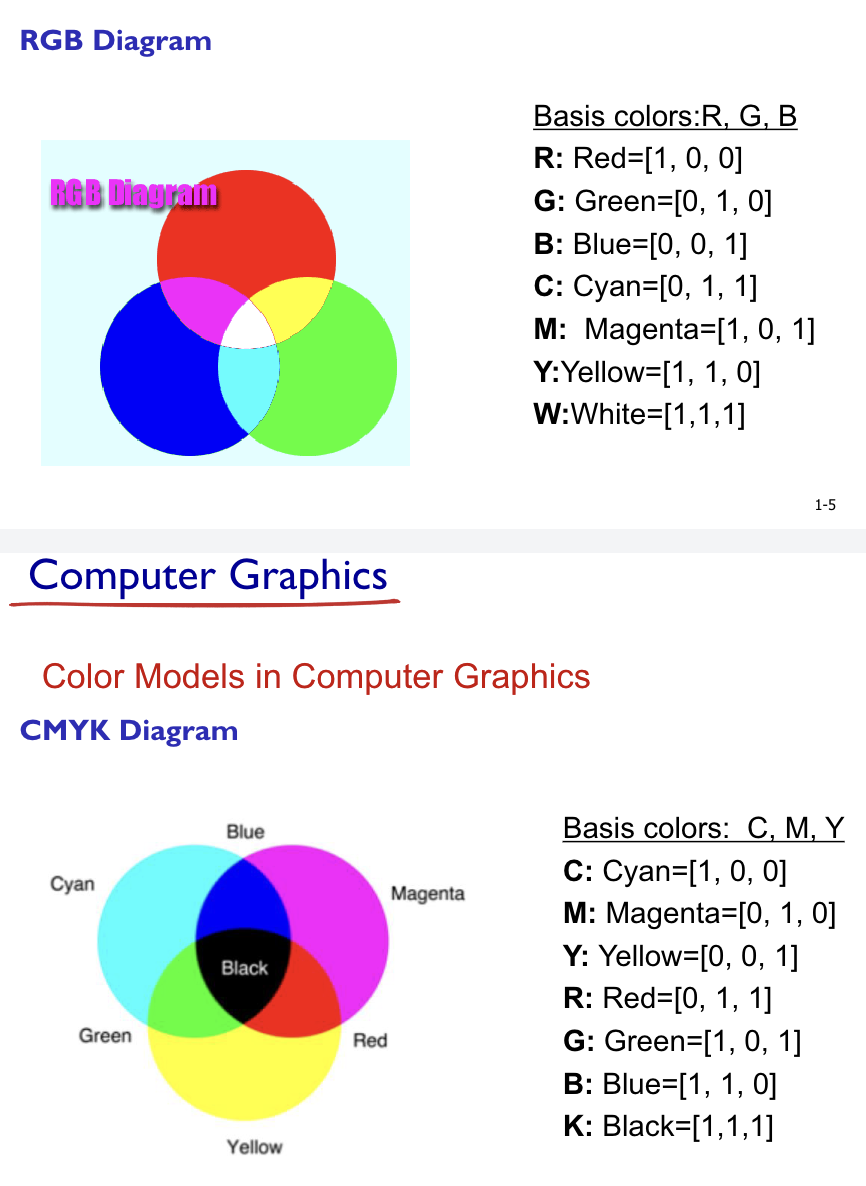
\includegraphics[width=0.7\textwidth]{static/ColorModel.png}
    \caption{ColorModel}
    \label{ColorModel}
\end{figure}

\subsection{图像表示}
\begin{itemize}
    \item 像素是图像的最小组成单位。
    \item The size of image 被定义为水平像素数量*垂直像素数量
    \item Aspect ratio of an image 图像的纵横比是高度与图像宽度比。
    \item 图像分辨率是一个单位的像素数量。
    \item JPEG，PNG，TIFF，GIF
\end{itemize}
\subsubsection{2-Dimention and 3-Dimention}
\begin{itemize}
    \item 2-Dimention 
    \begin{enumerate}
        \item 2维图像由一个有两个维度长度和宽度的平面进行表示。常常用于traditional printing, typography, drawing.
    \end{enumerate}
    \item 3-Dimention
    \begin{enumerate}
        \item 3维度图像由3个维度length width height进行表示。
        \item 3维图像是几何数据的表示
    \end{enumerate} 
    \item 2D vs 3D
        \begin{figure}[H]
            \centering
            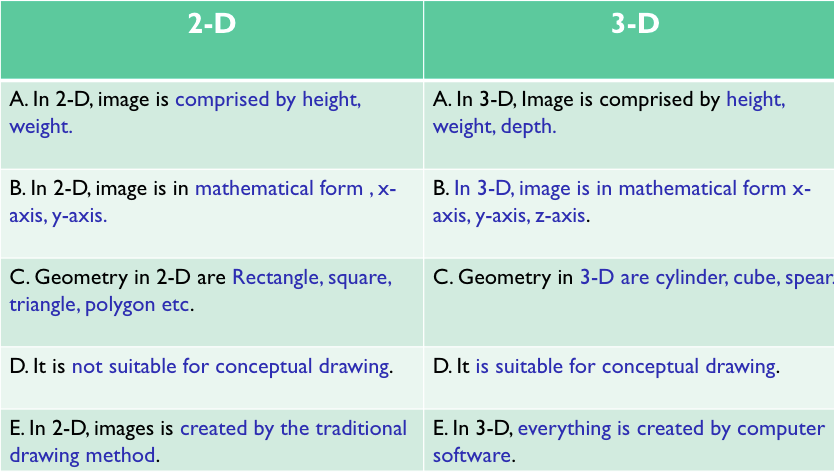
\includegraphics[width=0.7\textwidth]{static/2Dvs3D.png}
            \caption{2Dvs3D}
            \label{2Dvs3D}
        \end{figure}
\end{itemize}
\subsubsection{2-Dimention}
变换包括translation, rotation, reflection, scaling.
\begin{itemize}
    \item 2D Translation
    移动一个物体从一个位置到另一个位置。

    Translation distance pair $(T_x, T_y)$ is called translation vector/shift vector.
        \begin{figure}[H]
            \centering
            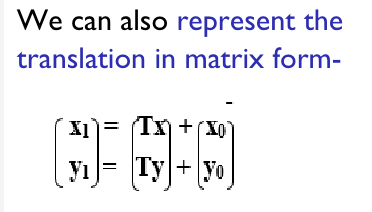
\includegraphics[width=0.7\textwidth]{static/2DTranslation.png}
            \caption{2DTranslation}
            \label{2DTranslation}
        \end{figure}

    \item 2D Scaling
    在二维平面上调整物体大小

    [Scaling of an Object= Original co-ordinates * Scaling Factors]

    \item 2D Rotation
    将物体从原点旋转到特定角度，

    旋转需要旋转点(pivot point)，旋转角$\theta$,旋转有两种方式clockwise(顺时针旋转，负的)和anti-clockwise(逆时针旋转，正的)。   
        \begin{figure}[H]
            \centering
            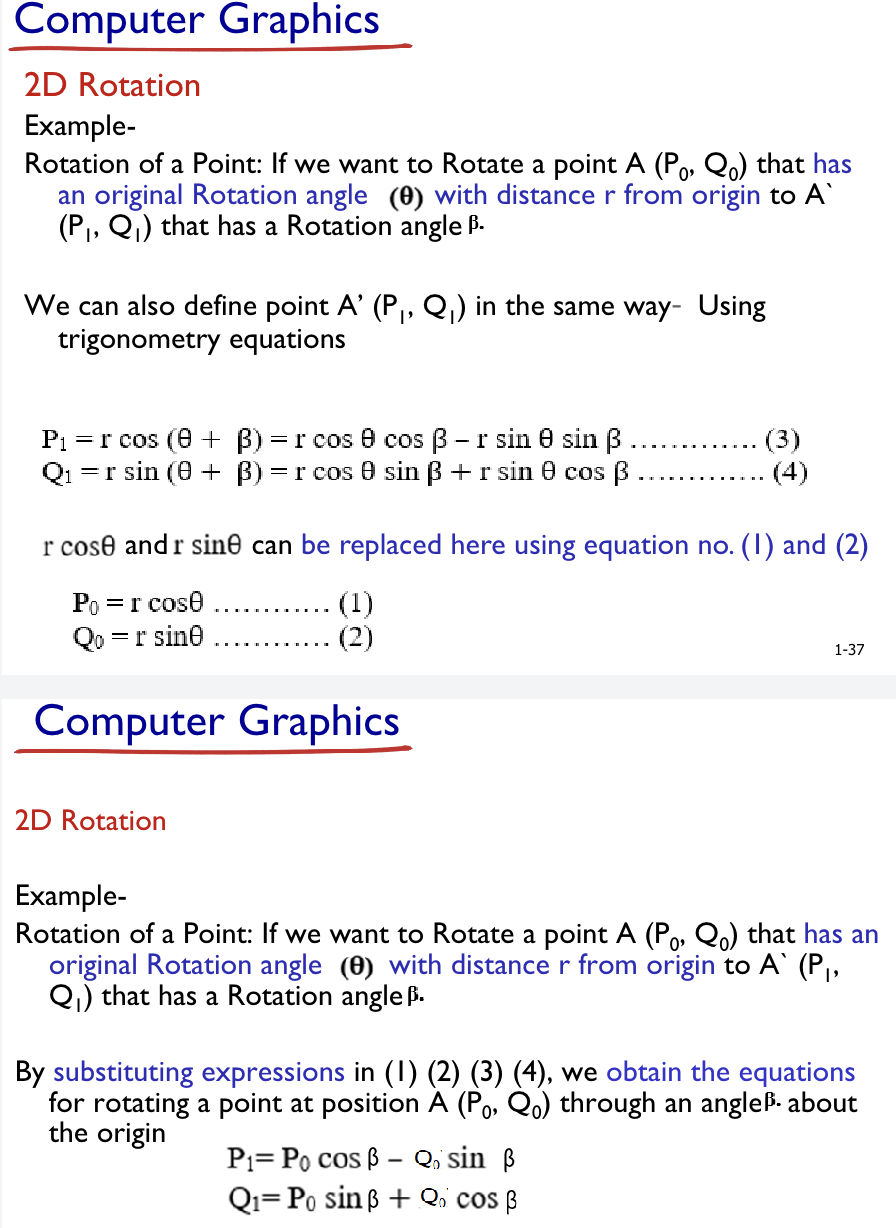
\includegraphics[width=0.7\textwidth]{static/2DRotation-induce.png}
            \caption{2DRotation-induce}
            \label{2DRotation-induce}
        \end{figure}
        \begin{figure}[H]
            \centering
            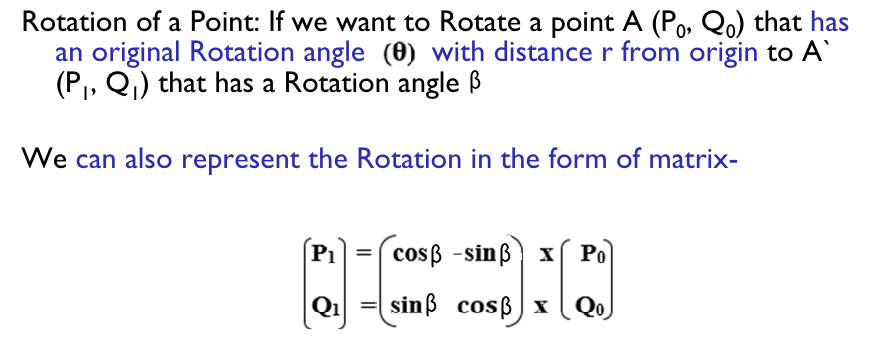
\includegraphics[width=0.7\textwidth]{static/2DRotation.png}
            \caption{2DRotation}
            \label{2DRotation}
        \end{figure}
    \item 2D Reflection
    Producing a mirror image of an object is called reflection.产生物体的镜像被称作反射。
    二维反射相对于一个轴生成镜像通过将物体绕着这个轴旋转180度。

    \begin{enumerate}
        \item 绕x轴反射
        \begin{figure}[H]
            \centering
            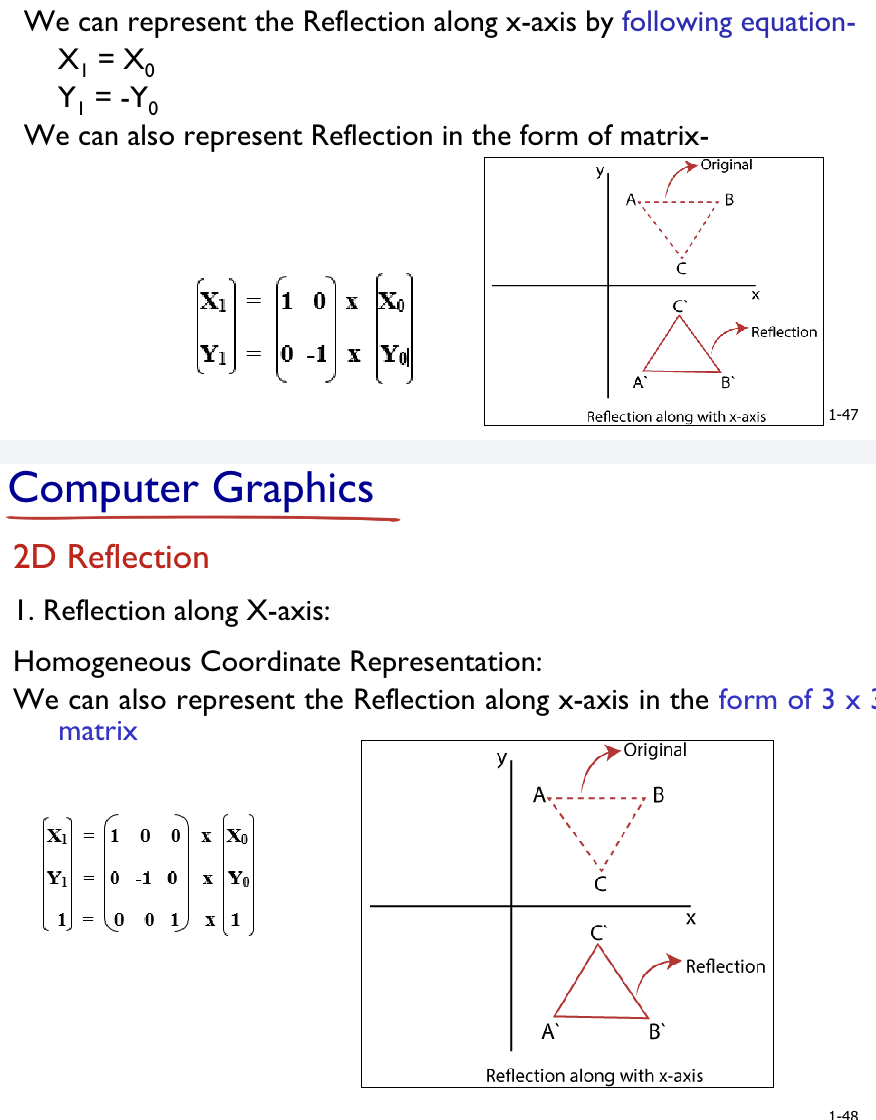
\includegraphics[width=0.7\textwidth]{static/X-axis-Reflect.png}
            \caption{X-axis-Reflect}
            \label{X-axis-Reflect}
        \end{figure} 
        \item 绕y轴反射    
        \begin{figure}[H]
            \centering
            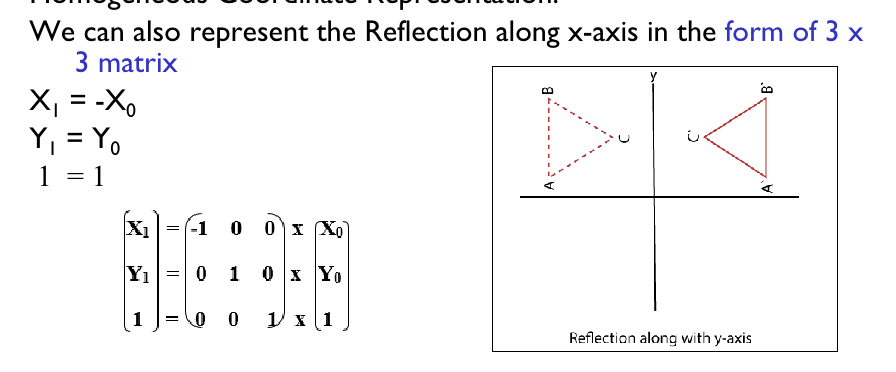
\includegraphics[width=0.6\textwidth]{static/Y-axis-Reflect.png}
            \caption{Y-axis-Reflect}
            \label{Y-axis-Reflect}
        \end{figure}  
        
        \item 绕垂直于XY的平面进行反射，也就是绕着原点旋转180度
        \begin{figure}[H]
            \centering
            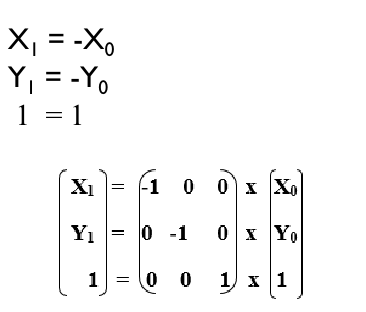
\includegraphics[width=0.6\textwidth]{static/PerpendicularXYPlant-Reflect.png}
            \caption{PerpendicularXYPlant-Reflect}
            \label{PerpendicularXYPlant-Reflect}
        \end{figure} 
        
        \item 沿y=x进行反射
        \begin{figure}[H]
            \centering
            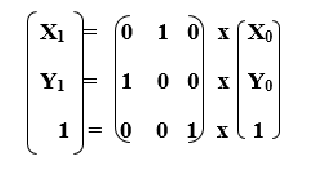
\includegraphics[width=0.6\textwidth]{static/YX-Reflection.png}
            \caption{YX-Reflection}
            \label{YX-Reflection}
        \end{figure} 
    \end{enumerate}
\end{itemize}

\subsubsection{3-Dimention Transformation}
\begin{itemize}
    \item 3D Translation
    
        \begin{figure}[H]
            \centering
            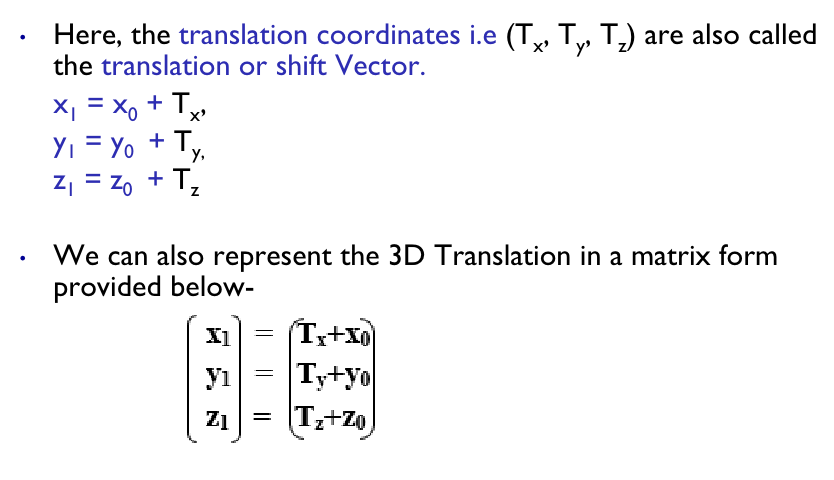
\includegraphics[width=0.6\textwidth]{static/3DTranslation.png}
            \caption{3DTranslation}
            \label{3DTranslation}
        \end{figure}

    \item 3D Scaling
        \begin{figure}[H]
            \centering
            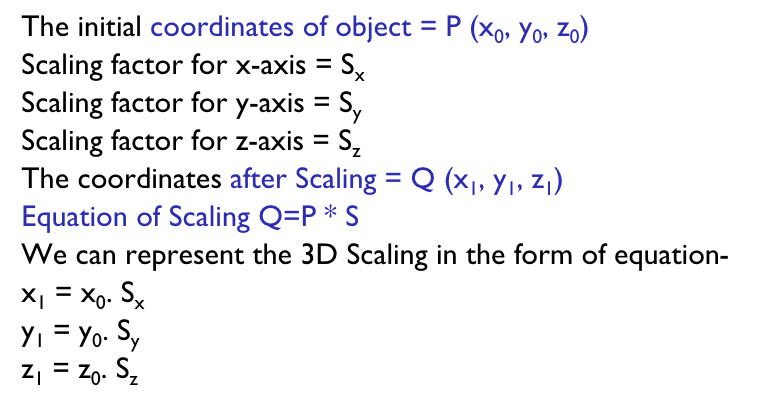
\includegraphics[width=0.6\textwidth]{static/3DScaling.png}
            \caption{3DScaling}
            \label{3DScaling}
        \end{figure} 

    \item 3D Rotation
    \begin{enumerate}
        \item X axis Rotation
            \begin{figure}[H]
                \centering
                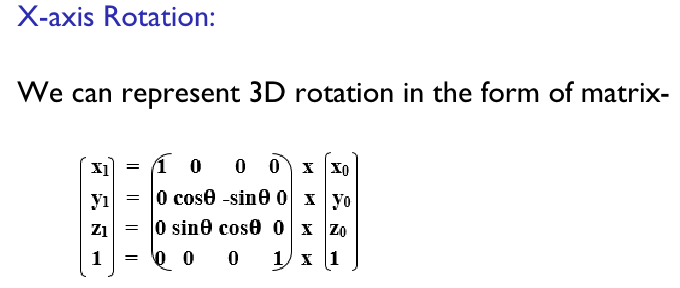
\includegraphics[width=0.6\textwidth]{static/3DX-Rotate.png}
                \caption{3DX-Rotate}
                \label{3DX-Rotate}
            \end{figure}
        \item Y axis Rotation
            \begin{figure}[H]
                \centering
                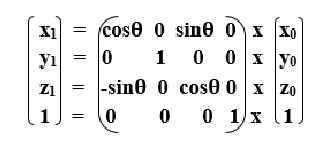
\includegraphics[width=0.6\textwidth]{static/3DY-Rotate.png}
                \caption{3DY-Rotate}
                \label{3DY-Rotate}
            \end{figure} 
        \item Z axis Rotation
            \begin{figure}[H]
                \centering
                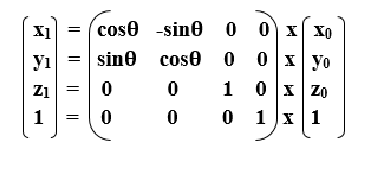
\includegraphics[width=0.6\textwidth]{static/3DZ-Rotate.png}
                \caption{3DZ-Rotate}
                \label{3DZ-Rotate}
            \end{figure} 
    \end{enumerate}
    
    \item 3D Reflection
    \begin{enumerate}
        \item XY Plane reflection
            \begin{figure}[H]
                \centering
                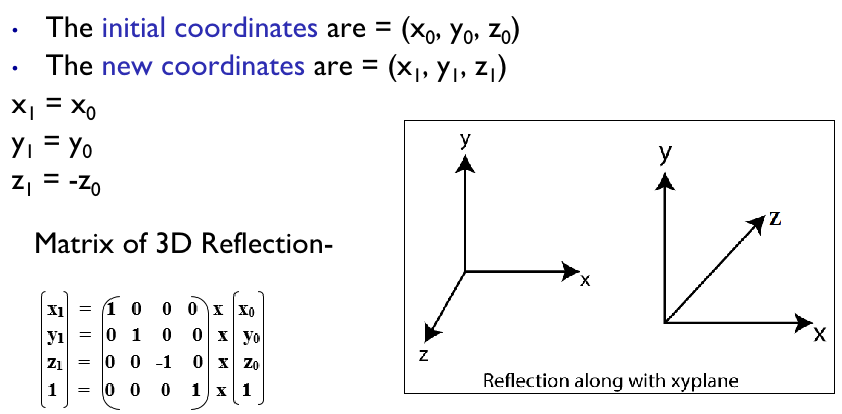
\includegraphics[width=0.6\textwidth]{static/3DXYPlane-Reflection.png}
                \caption{3DXYPlane-Reflection}
                \label{3DXYPlane-Reflection}
            \end{figure}
        \item XZ Plane reflection
            \begin{figure}[H]
                \centering
                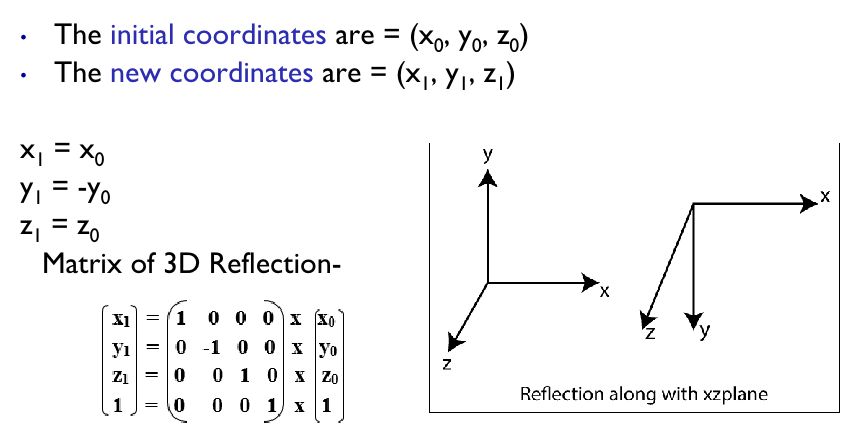
\includegraphics[width=0.6\textwidth]{static/3DXZPlane-Reflection.png}
                \caption{3DXZPlane-Reflection}
                \label{3DXZPlane-Reflection}
            \end{figure} 
        \item YZ Plane reflection
            \begin{figure}[H]
                \centering
                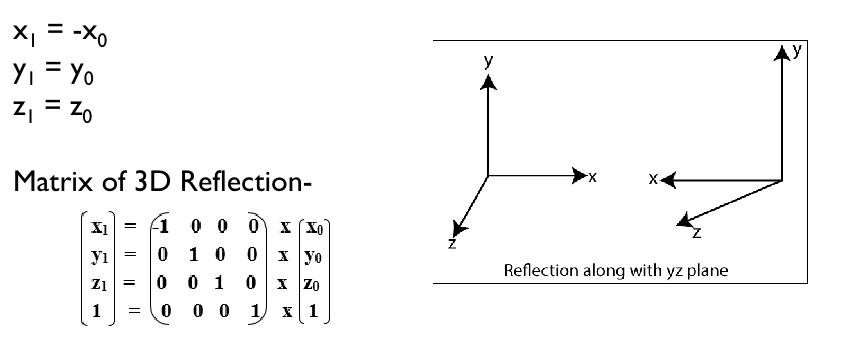
\includegraphics[width=0.6\textwidth]{static/3DYZPlane-Reflection.png}
                \caption{3DYZPlane-Reflection}
                \label{3DYZPlane-Reflection}
            \end{figure} 
    \end{enumerate}

\end{itemize}

\section{Chp3}

\subsection{Output Primitive输出图元}
输出图元是生成不同计算机图像对象的简单几何架构。
\begin{itemize}
    \item Point
    
    点是最基本的图像表示元素，是线的最小单位。

    \item Line
    
    线被定义为两个end point的连接

    \item Polyline折线
    
    折线是线段序列的连接，由N-1条线连接N个点，并且第一个点与最后一个点不连接，折线中的每一条线都被称为edge。

    \item polygon多边形
    
    多边形是一种闭合的图元，其使用N条线连接N个点，第一个点与最后一个点相连接。

    \item Filled Region 填充区域
    
    Filled region是一个帮助我们填充一个对象、区域或者图像的方法。
\end{itemize}

\subsection{Filled Algorithm填充算法}
\begin{itemize}
    \item Seed Fill Algorithm种子填充算法
    
    在种子填充算法中我们会在多边形的边界内选取一个起点叫做seed。
    \begin{enumerate}
        \item Flood-fill algorithm
        
        Flood-fill algorithm colors whole area through interconnected pixels by single color.类似于paint program中的bucket tools。
        \item Boundary-fill algorithm 
        
        先通过颜色或某个属性轮廓确定图像对象边界，在边界内部任意种子点出发，只在边界所包围的区域填充颜色。
    \end{enumerate}
    \item Scan Line Algorithm扫描线算法
    
    扫描线从上到下扫描图像，每次扫描线与图像多边形边界产生交点，将这些交点按照x坐标排序，将排序好的线段两两组成一个线段，并且使用对应颜色填充线段。
    
\end{itemize}

\subsection{Drawing Line Algorithm直线绘制算法}
$y=mx+c$, m是斜率，c是截距。$m=\frac{x_1-x_2}{y_1-y_2}$,$c=y-mx$
\begin{itemize}
    \item Digital differential analyzer数字差分分析仪
    
    首先，我们知道两个点$\text{起点}(x_0,y_0),\text{终点}(x_{k},y_{k})$,因此对于$m=\frac{y_{k}-y_{0}}{x_{k}-x_{0}}$
    我们分为3种情况：

    Case1:如果m<1,从k到k+1在x轴的改变量大于在y轴的改变量，因此设置$x_{k+1}-x_{k}=1$，此时根据斜率计算公式，$y_{k+1}-y_{k}=m$。

    Case2:如果m>1,从k到k+1在y轴的改变量大于在x轴的改变量，因此设置$y_{k+1}-y_{k}=1$，此时根据斜率计算公式，$x_{k+1}-x_{k}=\frac{1}{m}$。

    Case3:如果m=1,从k到k+1在y轴的改变量等于在x轴的改变量，因此设置$x_{k+1}-x_{k}=1$，$y_{k+1}-y_{k}=1$。

    \item Bresenham's Line Drawing 布雷森汉姆直线绘制算法
    
    首先，我们知道两个点$\text{起点}(x_0,y_0),\text{终点}(x_{k},y_{k})$,因此对于$\Delta y=y_{k}-y_{0}, \Delta x=x_{k}-x_{0}, m=\frac{\Delta y}{\Delta x}$

    计算decision parameter $ p_k=2\Delta y-\Delta x$.

    接下来分为2种情况：

    Case1:如果$p_{k}<0$,那么$x_{k+1}-x_{k}=1$,$y_{k+1}=y_{k}$,$p_{k+1}=p_{k}+2\Delta y$


    Case2:如果$p_{k}\geq 0$,那么$x_{k+1}-x_{k}=1$,$y_{k+1}-y_{k}=1$,$p_{k+1}=p_{k}+2\Delta y-2\Delta x$, 

    \item Mid point line Drawing 中点画线算法
    
    首先，我们知道两个点$\text{起点}(x_0,y_0),\text{终点}(x_{k},y_{k})$,因此对于$\Delta y=y_{k}-y_{0}, \Delta x=x_{k}-x_{0}, \Delta d=2(\Delta y-\Delta x)$

    计算decision paramete $d_{i}=2 \Delta y-\Delta x$

    2种情况：

    Case1:如果$d_{i}<0$,那么$x_{k+1}-x_{k}=1, y_{k+1}=y_{k}, d_{i+1}=d_{i}+2\Delta y$

    Case2:如果$d_{i}\geqslant 0$,那么$x_{k+1}-x_{k}=1, y_{k+1}-y_{k}=1, d_{i+1}=d_{i}+2\Delta d$

\end{itemize}

\section{Chp4}
\subsection{Clipping剪裁}
Clipping is a procedure that identifies which portions of a picture that are either inside or outside of our viewing pane.

选择用于显示图像的区域被称为窗口/剪裁窗口。

显示设备上用于映射窗口的区域被称为视图。

我们定义要显示图像所处的坐标系被叫作世界坐标系。

\subsection{Point Clipping 点剪裁}
点剪裁是确定点在视口内部或者视口外部的点过程。

假设我们有一个视口，X的范围$(xw_{min},xw_{max})$,Y的范围$(yw_{min},yw_{max})$,我们现在有一个点A(p,q),如何判断A是否在窗口里面？

如果$xw_{min}\leq p\leq xw_{max} $ and $yw_{min}\leq q\leq yw_{max} $, 那么点就落在视口之中，如果不满足以上条件，那么点就需要clipping。

\subsection{Line Clipping 线段剪裁}
线段剪裁是我们可以裁剪掉视口外部的线段，保留视口内部的线段。

一般过程：首先判断给定的线段是否完全在线段内部；如果不是的话，判断线段是否完全在视口外部；如果无法确定一条直线完全在内部或者外部，我们要计算一个或者多个裁剪边界的交点。

\subsubsection{Cohen Sutherland Line Clipping ALgorithm}
将view panel视角分为9个部分，从1到9是从左上到右下，使用4位二进制数对这9个部分进行表示，4位分别对应着上下右左。9个区域的区域5也就是中间是0000表示线段在这里面。

eg1:如果一条线的端点出现在右上角也就是区域3，那么对应的数字为1010。

\begin{itemize}
    \item 算法流程
    \begin{enumerate}
        \item 给线段的两个端点分配bit code
        \item 对两个端点的bit code做OR操作，如果结果为0000，那么线段在0000区域中，不用裁剪。
        \item 否则对两个端点取AND操作，
        \item 如果AND操作结果为0000，那么部分线段在视口区域中
        \item 否则，线段不再视口区域中
        \item 如果一条线需要被剪裁，需要找到这条线与4个边界的交点
        \item 如果这条线与左边界有交点，我们已知直线的斜率，并且已知左边界点的$xw_{min}$，我们可以通过斜率计算公式求出左边界点的y值。$y_{0}=y_{1}+m(x_{0}-x_{1})$.
        \item 如果这条线与右边界有交点，同理，$y_{0}=y_{1}+m(x_{0}-x_{1})$。
        \item 如果这条线与上边界有交点，$x_{0}=x_{1}+(y_{0}-y_{1})/m$
        \item 如果与下边界有交点，$x_{0}=x_{1}+(y_{0}-y_{1})/m$
    \end{enumerate}
\end{itemize}


\subsubsection{Liang-Barsky Line Clipping Algorithm}
\begin{itemize}
    \item 算法流程
    \begin{enumerate}
        \item 直线有两个端点, $(x_1,y_1)$ and $(x_2,y_2)$, $\Delta x=x_2-x_1, \Delta y=y_2-y_1$。$\Delta x>0$表示直线从左向右延伸，$\Delta y>0$表示直线从下向上延伸
        \item 计算方向参数$p_k$,直线相对于左边界水平方向$p_1=-\Delta x$若$p_1<0$那么直线由外向内走；直线相对右边界的水平方向$p_2=\Delta x$; 直线相对下边界的垂直方向$p_3=-\Delta y$,直线相对上边界的垂直方向$p_4=\Delta y$
        \item 计算距离参数$q_k$,起点到左边界的水平距离$q_1=x_1-xw_{min}$, 起点到右边界的水平距离$q_2=xw_{max}-x_1$，起点到上边界的垂直距离$q_3=yw_{max}-y_1$，起点到下边界的垂直距离$q_4=y_1-yw_{min}$
        \item 更新t的数值，t是time interval，开始$t_1=0$，结束$t_2=1$,从起点到终点。我们的坐标公式$x=x+t\Delta x$, $y=y+t\Delta y$
        \item 如果，我们遍历$p_k$，如果$p_k=0$，这一条直线与某一条边界平行，并且如果对应的$q_k<0$,那么这条平行线段在视口之外。
        \item 如果$p_k<0$线段从视口外向内走,$t_1=max(t_1,q_k/p_k)$,$q_k/p_k$计算进入时间。
        \item 如果$p_k>0$,$t_2=min(t_2,q_k/p_k)$，$q_k/p_k$计算离开时间从窗口内走出的时间。
        \item 如果$t_1>t_2$,进入时间大于离开时间，那么这条线不可视
        \item 否则$t_1<t_2$,计算剪裁后的端点;如果$t_1>0$,$x=x+t_1\Delta x$, $y=y+t_1\Delta y$,如果$t_2<1$,$x=x+t_2\Delta x$, $y=y+t_2\Delta y$,更新起点和终点。

    \end{enumerate}
\end{itemize}

\subsubsection{Midpoint Subdivision Line Clipping Algorithm 中点割线裁剪算法}
\begin{itemize}
    \item 算法流程
    \begin{enumerate}
        \item 像Cohen Sutherland Clipping Algorithm为线段两个端点分配bit code。
        \item 两个端点的bit code实现OR操作，如果OR操作结果为0000，则线段在视口内；
        \item 否则，对两个端点实现AND操作，如果AND操作不为0000，则线段在视口外不可见，如果AND为0000，则线段部分在视口内部分在视口外
        \item 对于部分可见的线段，使用$X_m=(x_1+x_2)/2, Y_m=(y_1+y_2)/2$求线段中点。要知道两个端点在窗口内还是窗口外。我们求出的中点如果在窗口内，那么我们要把窗口内的端点更新到此中点；如果求出来的中点在窗口外，那么要把窗口外的端点更新到中点的位置。
    \end{enumerate}
\end{itemize}

\subsection{Polygon Clipping 多边形剪裁}
A polygon can be described as the enclosed collection of the lines.

\subsubsection{Sutherland-Hodgeman polygon clipping algorithm}
\begin{itemize}
    \item 算法流程
    \begin{enumerate}
        \item 多边形剪裁算法要处理4种不同的剪裁情况，包括左剪裁，右剪裁，上剪裁，下剪裁。在对每一种情况进行剪裁时，我们移除某一个部分在视口外的区域，保留视口内的区域。比如在左剪裁中，我们只移除多边形左侧位于窗口外部的部分，保留窗口内部的部分。
        \item 在做每一个case时，多边形的每一条边$v_1=(x_1,y_1),v_2=(x_2,y_2)$，我们要考虑4个conditions，并且我们需要使用列表存储多边形的顶点和交点
        \item 如果边是从外部到内部，那么多边形的边和边界的交点记为$v^{'}_1$,列表中需要存储$v^{'}_1$和$v_2$
        \item 如果边是从内部到内部，那么列表要存储$v_2$
        \item 如果边是从内部到外部，那么列表要存储$v^{'}_1$,
        \item 如果边是从外部到外部，则不用存储任何信息
    \end{enumerate}
\end{itemize}

\subsubsection{Weiler-Atherton polygon clipping algorithm}
\begin{itemize}
    \item 算法流程
    \begin{enumerate}
        \item 首先，创建一个用于标识进入窗口或者退出窗口状态的交点列表。
        \item 接着，创建一个包含all the vertices of the polygon 在subject polygon list；以及一个剪裁窗口点点Clip Polygon List，刚开始按顺时针存储着剪裁窗口的点。
        \item 遍历subject polygon list中的按顺序的两个点可以组成的边E，并且遍历剪裁窗口中按顺序的两个点组成的边C是否与E相交，如果相交计算交点坐标，并且标记交点是入窗口还是出窗口以及其前驱和后继，并且将交点插入在E边和C边组成的交点之间。
        \item 从第一个进入点开始走，沿着主多边形列表走，直到遇到离开点，切换到剪裁窗口列表并且找到离开点，然后沿着剪裁窗口走，遇到进入点切换回主多边形列表，循环直到回到原点。
    \end{enumerate}
\end{itemize}


\subsection{Text Clipping文本剪裁}
Text clipping is a process in which we remove the part of the string that is outside of the view pane.

\subsubsection{All-or-none string-clipping 全有或者全无字符串剪裁}
如果环绕在字符串矩形边界框与窗口边界有重叠，那么这个字符串直接被rejected（直接消失），这也是最快的文本剪裁方法。


\subsubsection{All-or-none character-clipping 全有或者全无字符剪裁}

\begin{itemize}
    \item Rejecting an entire character
    
    单个字符的边界将会与窗口进行比较，如果字符边界与窗口边界重合或者位于窗口边界之外，此字符将会被剪裁。

    \item CLip the components of individual characters
    
    如果单个字符与剪裁窗口重合，那么剪裁掉该字符位于窗口之外的部分。

    一般来说如果是由线段构成的轮廓字符可以使用这种方法进行剪裁。
\end{itemize}

\section{Chp5}
\subsection{Rendering}
Rendering is an automatic process of creating digital image from a template by using software system.

\begin{itemize}
    \item Rendering real time
    
    Real-time rendering is a process where the image is produced and analyzed from 3D information at a fast speed.
    \item Render offline
    
    Offline rendering is a technique mainly used in situations where the processing speed is slow.
\end{itemize}

\subsubsection{Rendering techniques}
\begin{itemize}
    \item Z-Buffer
    \begin{enumerate}
        \item Z-Buffer is also called Depth Buffer, which is used for hidden surface detection. And Z-Buffer means a memory area that keeps z coordinates and intensity closest to the observers for each pixel.
        \item Depth buffer requires 2 arrays.One is for keeping the intensity of the pixel, another one records z value. 
    \end{enumerate}
    \item Scan line
    \begin{enumerate}
        \item Scan line is used for determining the visible surfaces one line at a time.
        \item Scan line keeps the records of two edge lists. One is edge list which contains the coordinates of two endpoints of a edge. Other one is active edge line(AEL), it contains the edges that intersects with scan line during it sweeps.
    \end{enumerate}
    \item Hidden Line Rendering
    
    Hidden line rendering is used to represent object whose surface is covered and blocked with lines representing the sides of the object.

    \item Ray tracing rendering
    
    Ray tracing rendering follows the light on its way from the light source to the screen and estimates what kind of color is displayed on the pixel where the ray falls.

    The ray tracing rendering builds an image by extending rays into a scene.
    
\end{itemize}

\subsubsection{Features of rendering}
\begin{itemize}
    \item Shading着色
    
    Shading is an appearance of lights and darks found in a surface of an object.
    \item Texture mapping纹理映射
    
    Texture mapping is a graphics design procedure, that refers to the pattern of the surface.
    \item Bump mapping凹凸映射
    
    Bump mapping is a process that visualizing slight bumpiness on layers.
    \item Motion blur运动模糊
    
    Motion blur is caused by relative motion between image acquisition system and an object, and items appear blurry due to the increased movement or the movement of the camera.
\end{itemize}

\subsection{Animation}
Animation refers to any time sequence of visual changes in pictures, including size, shape, color, structure, angle.

\subsubsection{Animation Function}

\begin{itemize}
    \item Morphing(变形)
    
    变形包括3个过程：
    \begin{enumerate}
        \item One initial image and final image as two key frames are added the morphing application.
        \item The selection of key points on both the images for a smooth transition between two images.
        \item The key point of the first image transforms to the corresponding key points of the second image.
    \end{enumerate}

    \item Panning(平移)
    \begin{enumerate}
        \item Panning refers to the movement of the fixed size window across the window object in a scene. And the direction in which the fixed size window moves, the window objects moves in opposite direction.
    \end{enumerate}
    \item Zooming(缩放)
    \begin{enumerate}
        \item In zooming, the window is fixed an object and changes its size. The objects also appear to change in size.
        \item Zooming In and Zooming Out are used to enlarge and reduce the size of the view.
    \end{enumerate}
    \item Fractals(分形)
    \begin{enumerate}
        \item Fractal function is used to generate the complex picture by the repetition of a single formulas again and again with a slightly different value.
    \end{enumerate}
\end{itemize}

\subsection{Light Source}

\begin{itemize}
    \item Lighting model/ illumination model is used to calculate the intensity of light that is reflected at a given point on the surface.
    \item Lighting effect depends on 3 factors:
    \begin{enumerate}
        \item light source 
        \item surface 
        \item observers
    \end{enumerate}
    \item 3 Types of Light source 
    \begin{enumerate}
        \item Point sources
        \begin{itemize}
            \item Point sources emit light from a single point in all directions.
            \item The intensity of the point light decreasing with distance.
        \end{itemize}
        \item Parallel sources
        
        Parallel sources can be considered as a point source which is far from the surface.

        \item Distributed sources
        
        Rays originates from a finite area.

    \end{enumerate}
    \item Reflection
    
    When the light falls on the surface, the light gets absorbed and reflected. And the surface structure decides the amount of reflection and absorbed.

    The observer's position and sensor spectrum sensitivities also affect the lightning effect.


    \begin{itemize}
        \item Diffuse reflection漫反射
        
        Diffuse reflection occurs on the surface which are rough.

        $I=I_p K_d cos(\theta)=I_p K_d (N^{'}*L^{'})$
        \begin{enumerate}
            \item I是漫反射光照强度
            \item $I_p$是光源光照强度
            \item $K_d$是漫反射系数,从0到1 for each RGB
            \item $N^{'}$是normalized surface，物体表面某点的单位法向量
            \item $L^{'}$是指向光源的normalized direction单位向量。
        \end{enumerate}
        
        \item Spectrum reflection 镜面反射
        
        Spectrum reflection occurs on when light falls on shiny surface.

        Phone Model

        $I=I_p cos^n(a) W(\theta)$
        \begin{enumerate}
            \item n 是specular-reflection exponent
            \item a 是观测者视线与反射光线的夹角
            \item $W(\theta)$是镜面反射系数
        \end{enumerate}

        \item Ambient环境光
        
        Ambient is non-directional light source and not affected by anything in the world.

        $I=I_a K_a$
        \begin{enumerate}
            \item $I_a$是环境光强度
            \item $K_a$是环境光反射系数
        \end{enumerate}

    \end{itemize}

    \item Shading model
    
    Shading refers to the process of altering the color of the object in 3D scene.
    影响着色效果的因素：the surface's angle to the light, the distance from lights, its angle to the camera and material property.

    由于我们经常使用大量的多边形去模拟曲面，因此我们希望相邻的多边形颜色可以平滑地过渡。
    \begin{enumerate}
        \item Flat shading 平面着色
        
        In flat shading, all points over the surface of the polygon are displayed with the same intensity value.

        \item Color interpolation shading/ Goraud shading

        如果我们知道两个点的intensity那么我们能够知道这两个点之间任何一个点的强度。

        \item Normal interpolation shading/ Phong shading
        
        颜色差值着色需要知道多边形每个顶点的法向量，时间成本比线性差值更高。

    \end{enumerate}

\end{itemize}

\end{document}